%Having Nek's mathematical description of \sref{math} in mind, we can see that modern compilers 
%and math libraries are challenged by Nek's small matrix products and non-temporal vector and element
%updates. 
%In the following paragraphs we address the optimizations of both and close this section by a performance
%discussion of the previously identified matrix-matrix kernels carried out via proxy applications. 

\subsection{Small Matrix Multiplications}

The implementation of fast matrix multiplications, i.e., the BLAS library's GEMM routines, and dense linear algebra more generally is one of computer science's best studied fields. 
However, large matrices~\cite{Goto:2008:AHM:1356052.1356053} have been the primary focus and, as a result, vendor-tuned BLAS implementations do not provide optimal performance when used for the small GEMMs in Nek. 
Several BLAS libraries recently introduced so-called batched interfaces to speed-up series of independent and small multiplications by exploiting parallelism and amortizing calling overheads~\cite{mklbatch}. 
As Nek performs dependent GEMMs within each element, batched execution would necessarily be inter-element,  inhibiting important caching optimization and consuming significantly more memory bandwidth. 
Therefore, most of Nek's computer science related work was devoted on speeding up small GEMMs~\cite{Shin:2010:SUN:1810085.1810120}.
Parts of Nek5000 and the related NekCEM codes have been independently ported to OpenACC~\cite{markidis2015openacc, otten2016} to speed-up small GEMMs.

Today, Nek5000 and NekBox ship with a FORTRAN-based matrix-matrix implementation called \texttt{mxm\_std}.
By default, \texttt{mxm\_std} explicitly defines multiple interfaces corresponding to values of the inner dimension $k$, and provides unrolled FORTRAN primitives to the compiler.
 For IBM's BlueGene series, common sizes are manually implemented for best performance in FORTRAN assembly-intrinsics in \texttt{mxm\_bgq}. 
Similarly, \texttt{mxm\_std} features some special case optimizations targeting AMD's Opteron processor, which is used in the United States' largest system, Titan, at Oak Ridge National Laboratory.

In order to ensure the best possible performance on a range of modern Intel processors, featuring different versions of Advance Vector Extensions (AVX) instructions, we would need to conduct a long and complicated tuning effort of Nek's \texttt{mxm\_std} akin to the narrow customizations already present.
Instead, we integrated an early prototype of the LIBXSMM library~\cite{LIBXSMM,sc15poster} into NekBox. 
LIBXSMM provides highly-optimized single-threaded small matrix-multiplication routines tuned for all recent Intel processors. 
It is already successfully used in the quantum chemistry application CP2K and high-order finite element seismic wave equation solver SeisSol~\cite{breuer15high-order}. 

In contrast to \texttt{mxm\_std}, LIBXSMM creates a specific kernel implementation for each small matrix multiplication size and optimizes that kernel specifically for each set of vector extensions.
Each kernel is composed from a-priori known and best-performing basic blocks.  
Remainder handling can be performed either explicitly by application-side padding or internally by slightly less efficient fill-in basic blocks. 
We rely on the latter in our integration of LIBXSMM into NekBox. 

We leverage LIBXSMM's experimental just-in-time (JIT) compilation feature to adapt at runtime to Nek's spectral order. 
The JIT feature generates a small matrix multiplication when its size is requested for the first time and caches compiled code until the application process is terminated. 
Additionally, LIBXSMM can expose the function pointer to the application to bypass future dispatches when call patterns are simple. 

As an example, we provide the integration of LIBXSMM into NekBox's local Helmholtz kernel from \sref{operators} in \lref{int_axhm}.
This fragment is called within a loop over elements that is typically long enough to amortize overheads. 
When entering the element-local operator for the very first time, we request the required kernels from the LIBXSMM library, which JIT compiles them internally, and store the corresponding functions pointers into persistent variables to avoid dispatching in subsequent calls. 
Compared to the pseudo-code fragment, cf.~\ref{sec:operators}, we use temporary buffers to separate matrix-matrix from vector-vector operations, which are performed in one step at the end of each element.
The other common matrix-matrix motifs, basis transformation in particular, are optimized analogously. 

\begin{lstlisting}[float,
  caption={Integration of LIBXSMM into NekBox's element-local Helmholtz operator. \texttt{xmm1, xmm2, xmm3} are persistent
  functions pointers to amortize LIBXSMM's dispatching overhead. The \texttt{libxsmm\_dispatch} call JITs the requested kernel and 
  populates the persistent function pointers.},
  label=lst:int_axhm]
  logical, save :: init = .false.
  type(LIBXSMM_DMM_FUNCTION), save :: xmm1, xmm2, xmm3

  ! lazy initialization of function-private function pointers
  ! to eliminate dispatching overhead
  if (.not. init) then
    call libxsmm_dispatch(xmm1, nx, ny*nz, nx, 1.0_dp, 0.0_dp)
    call libxsmm_dispatch(xmm2, nx, ny, ny, 1.0_dp, 0.0_dp)
    call libxsmm_dispatch(xmm3, nx*ny, nz, nz, 1.0_dp, 0.0_dp)
    init = .true.
  endif

  ! element-local operation
  call libxsmm_call(xmm1, C_LOC(wddx), C_LOC(u(1,1,1)), C_LOC(work1))
  do iz=1,nz
      call libxsmm_call(xmm2, C_LOC(u(1,1,iz)), C_LOC(wddyt), C_LOC(work2(1,1,iz)))
  enddo
  call libxsmm_call(xmm3, C_LOC(u(1,1,1)), C_LOC(wddzt), C_LOC(work3))

  ! element update
  au(:,:,:) = h1* ( work1*gx + work2*gy + work3*gz ) + h2*b*u
\end{lstlisting}

\subsection{Enhancing Element Update Performance by Streaming Stores}
Caches in Intel processors are designed as write-back caches with read-for-ownership (RFO).
Therefore, writing to a vector in main memory costs two operations: a load into the cache and the write.
Nek performs many such element updates, cf. \lref{int_axhm}, and long vector updates in linear solvers.
Compiling the Helmholtz element update leads to 5 streams being
explicitly read (\texttt{gx, gy, gz, b, u}), one RFO of \texttt{au} and one write of \texttt{au}. As we stream through all elements
the RFOs are harmful for two reasons: a) they consume bandwidth
and therefore can cause a $\approx$ 16\% performance drop; 
and b) they unnecessarily occupy cache space and might  
evict useful data. 

Since the SSE2 instruction set, the Intel architecture offers so-called non-temporal stores (NTS).
These special instructions write data directly into main memory without generating RFOs and consuming cache.
They operate best when being executed on vector-length aligned addresses, as cache-line splits are impossible. 
The compiler cannot fulfill the alignment requirement for all orders, because Nek stores field data compactly, which prohibits semi-automatic generation of NTS.
Therefore, we implemented a FORTRAN interface module with a C-backend and x86 intrinsics that applies loop-peeling to leverage
NTS for the majority of stores in long, potentially unaligned updates. 
This module covers the important kernels of Nek by offering NTS-enhanced primitives to: a) set an 1d-array to a fixed value b) copy an 1d-array c) multiply component-wise an 1d array, and d) perform the Helmholtz element update, including the special case of the Poisson operator, $h_2 = 0$. For case b), Listing~\ref{lst:streamcopy} depicts Intel AVX2 code.

\begin{lstlisting}[
  float,
  language=C++,
  label={lst:streamcopy},
  caption={Loop peeling approach including determining the middle section for which aligned NTS instructions can be used.}
]{}
void stream_vector_copy( const double* i_a,
                         double*       io_c,
                         const int     i_length) {
  int l_n = 0;
  int l_trip_prolog = 0;
  int l_trip_stream = 0;
  
  /* init the trip counts to determine aligned middle section */
  stream_init( i_length, (size_t)io_c, &l_trip_prolog, &l_trip_stream );

  /* run the prologue */
  for ( ; l_n < l_trip_prolog;  l_n++ ) {
    io_c[l_n] = i_a[l_n];
  }
  /* run the bulk, using streaming stores */
  for ( ; l_n < l_trip_stream;  l_n+=8 ) {
    _mm256_stream_pd( &(io_c[l_n]),   _mm256_loadu_pd(&(i_a[l_n]))   );
    _mm256_stream_pd( &(io_c[l_n+4]), _mm256_loadu_pd(&(i_a[l_n+4])) );
  }
  /* run the epilogue */
  for ( ; l_n < i_length;  l_n++ ) {
    io_c[l_n] = i_a[l_n];
  }
}
\end{lstlisting}

\subsection{Discussion of Performance Reproducers}
In order to analyze the performance of LIBXSMM integration and the NTS module,
we have implemented standalone reproducers of the identified small matrix multiplication motifs. 
They are included in the LIBXSMM library as examples and performance tests.
In contrast to NekBox, they are parallelized via OpenMP instead of MPI, but the performance agrees within 10\% of a full NekBox execution at scale. 
We used a single node of the Cray XC40 and BlueGene/Q, cf. \sref{arch}, for generating performance data in this section.

\fref{axhm} compares the performance of Intel MKL 11.2.1, Nek's own \texttt{mxm\_std}, and LIBXSMM
with and without non-temporal stores. 
For all element sizes, LIBXSMM offers the best performance, but the difference for orders $\leq 16$ are very small as the execution is heavily memory bandwidth bound. 
A significant boost is possible by leveraging NTS: we are able to sustain 100\% of the STREAM triad 
bandwidth (101.6\,GiB/s) up to an element size of 16. 
For larger problems, the small GEMM performance is more important. 
Here LIBXSMM is up to 2$\times$ faster than \texttt{mxm\_std} und up to 40\% faster than Intel MKL. 

In case of very low orders the benefit of NTS is greater than 16\%, which we attribute to NTS avoiding cache pollution. 
For medium sized orders we exactly see the expected 16\%,
and large problems have additional bandwidth available such that RFOs are less harmful.
 
\begin{figure}[!t]
\centering
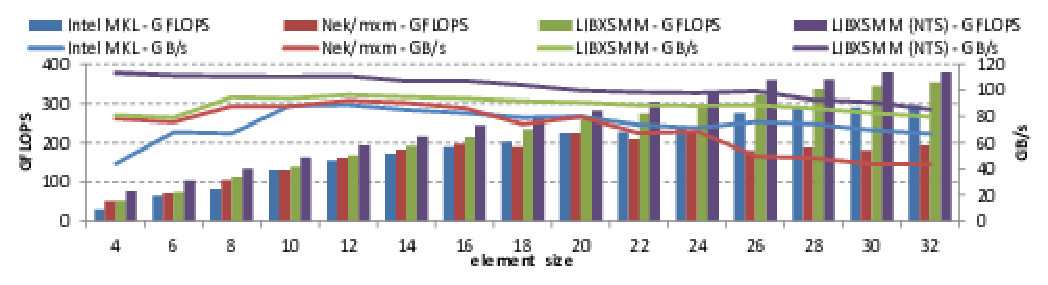
\includegraphics[width=1.0\textwidth]{gfx/axhm}
\caption{
Performance of the Helmholtz reproducer running on a single node of Shaheen for different implementation of small matrix multiplications. 
NTS denotes the usage of the non-temporal store optimized module.}
\label{fig:axhm}
\end{figure}

The performance numbers for the basis transformation on Shaheen are comparable to the Helmholtz operator and 
therefore not plotted. 
To summarize them, LIBXSMM-based GEMMs are the fastest and, due to higher computational demand, NTS are only important of for very small 1d sizes.
LIBXSMM is able to achieve 50\% of maximum floating-point performance for moderate orders.
LIBXSMM ranges from 4$\times$ faster than \texttt{mxm\_std} and Intel MKL at the smallest order to 40\% faster at the largest.


The performance of the Helmholtz kernel is representative of the basis transformations kernel on Mira as well.
To compare with Shaheen, \fref{axhm_mira} repeats the Helmholtz operator reproducer experiment
on a single node of Mira. 
IBM ESSL version 5.1.1 is used as the vendor library in place of Intel MKL.
In place of LIBXSMM, \texttt{mxm\_bgq}, which features QPX SIMD instructions, is used for the sizes that it supports.
When no QPX implementation is available, \texttt{mxm\_bgq} falls back to \texttt{mxm\_std}. 
Up to element size 16, Nek's \texttt{mxm\_std} and \texttt{mxm\_bgq} libraries are a better choice compared to IBM ESSL.
For larger element sizes (except 22 and 24) the performance is comparable.
However, the fraction of available bandwidth used is significantly worse than on Shaheen. 
Even at high element sizes, Shaheen is at 80\% bandwidth utilization with LIBXSMM and 50\% without, whereas Mira runs at 17\%.
The relative efficacy of \texttt{mxm\_bgq} on Mira, where available, highlights the strength of LIBXSMM: the ability to automatically issue the best available vector instructions at any size.


\begin{figure}[!t]
\centering
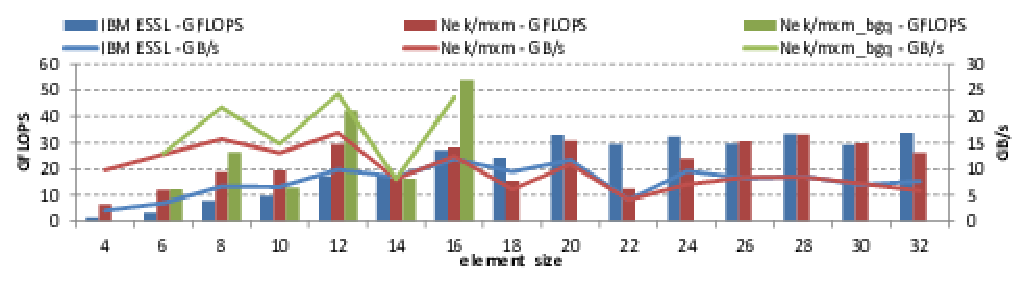
\includegraphics[width=1.0\textwidth]{gfx/axhm_mira}
\caption{
Performance of the Helmholtz operator reproducer running on a single node of Mira for different implementation of small matrix multiplications.}
\label{fig:axhm_mira}
\end{figure}

\fref{rstr} depicts corresponding performance numbers for the basis transformation reproducer in three use cases: a) unitary transformation from element size to element size, b) prolongation/dealiasing from 1d size to $(3/2)$ the element size, and c) restriction/aliasing from 1d size to (2/3) the element size.
Note that the $(3/2)$ factor implies some dimensions are significantly larger then the element size shown on the x-axis.

As with the Helmholtz reproducer, the LIBXSMM-based executions are the fastest and due to higher
computational demand; 
NTS are only important of for very small 1d sizes. 
LIBXSMM is able to achieve 50\% of maximum floating-point performance for medium sized orders
In direct comparison to \texttt{mxm\_std} and Intel MKL, the speed-up of LIBXSMM varies between close to 4$\times$ at very small order to roughly 40\% at very large order.

\begin{figure}[!t]
\centering
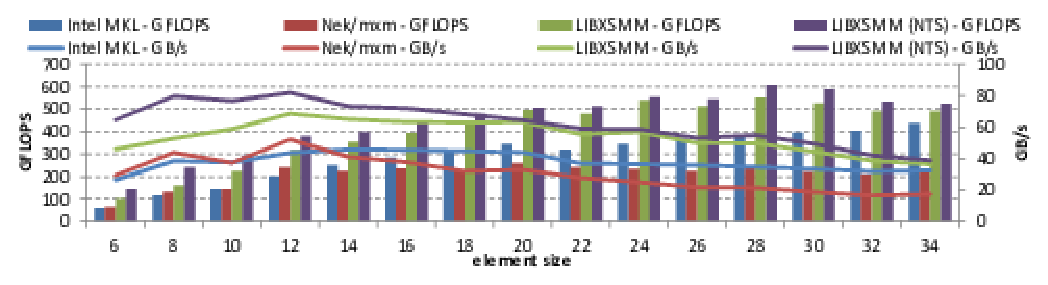
\includegraphics[width=1.0\textwidth]{gfx/rstr}   
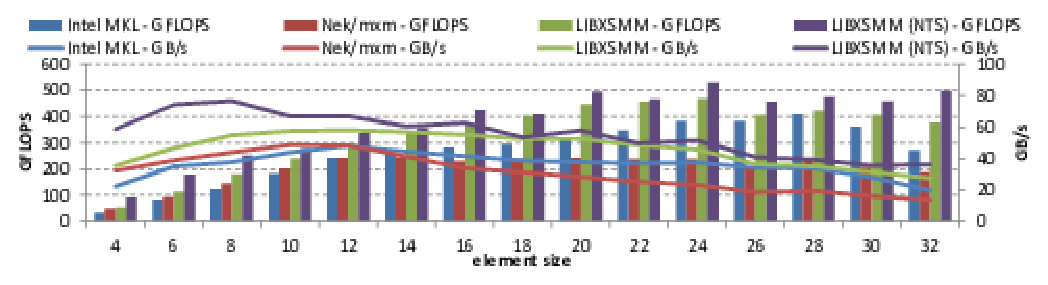
\includegraphics[width=1.0\textwidth]{gfx/rstr_fwd}
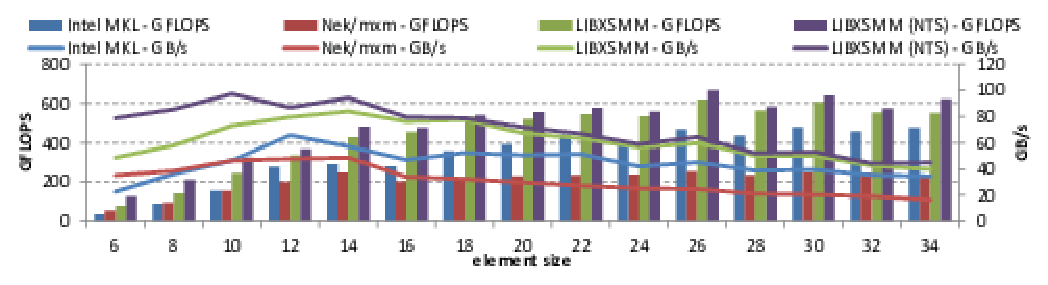
\includegraphics[width=1.0\textwidth]{gfx/rstr_rev}
\caption{Performance of the basis transformation reproducers using different implementation for the 
small matrix multiplications. NTS denotes the usage of the aforementioned non-temporal store optimized module. The top plot
shows the diagonalization in the local Poisson operator, the middle one the prolongation and the bottom one the restriction case.}
\label{fig:rstr}
\end{figure}

%Finally, the gradient reproducer's performance is plotted in \fref{grad}.
%The floating point load is very similar to Helmholtz, but only one element is read, instead of five, and three elements are written, %instead of one.
%While both are bandwidth bound, the higher write load makes gradient more sensitive to RFO.
%NTS doubles the performance in case of small and medium sized orders. 
%Therefore, without NTS, the high bandwidth cost masks the floating point cost and it does not matter which matrix-matrix routines are %used.
%Even so, LIBXSMM results in the fastest execution.
%
%\begin{figure}[!t]
%\centering
%\includegraphics[width=1.0\textwidth]{gfx/grad}
%\caption{Performance of the gradient operator reproducer using different implementation for the small matrix 
%multiplications. NTS denotes the usage of the aforementioned non-temporal store optimized module.}
%\label{fig:grad}
%\end{figure}
